\section{Introduction}
\label{sec:introduction}
\subsection{What is Machine Learning?}
\label{subsec:introduction-definition}
\begin{frame}{\insertsubsection}
    'A computer program is said to learn from experience $E$ with respect to some class of tasks $T$ and performance measure $P$ if its performance at tasks in $T$, as measured by $P$, improves with experience $E$'\\
    - Tom M. Mitchell~\cite{Mitchell1997}
\end{frame}
%
%
\subsection{History of Machine Learning}
\label{subsec:introduction-history}
\begin{frame}{\insertsubsection}
    \begin{itemize}[<+->]
        \item[1943] First publication of neural network~\cite{McCulloch1943}
        \item[1956] Dartmouth Summer Research Project (Birthplace of modern Machine Learning)
        \item[1965] Nilson Machine Learning for pattern classification~\cite{Nilsson1965}
        \item[1966] Following years: Many setbacks in Artificial Intelligence called 'AI-Winters'
        \item[1995] Support Vector Machines are first introduced
        \item[2002] Torch first release (open source library)
        \item[2006] Geoffrey Hinton coins 'Deep Learning'~\cite{Hinton2006}
        \item[>2006] Companies such as Netflix, Facebook, Microsoft, Google fund projects/prizes in and use machine learning/artificial intelligence
    \end{itemize}
\end{frame}
%
%
\subsection{Workflow}
\label{subsec:introduction-workflow}
\begin{frame}{\insertsubsection}
    Machine learning techniques follow a similar workflow.
    \begin{enumerate}[<+->]
        \item Define Problem (scope, feasability)
        \item Gather Data (assumptions, constraints)
        \item Pre-process Data (cleanup, drop)
        \item Analyze Data (define features, find correlations)
        \item Prepare Data (transform, normalize, drop)
        \item Evaluate Models (train/test, classify/regress)
        \item Tune Model (cross validation, fine tune parameters)
        \item Apply model to problems, learn more
    \end{enumerate}
\end{frame}
%
%
\begin{frame}{\insertsubsection}
    \begin{figure}
        \centering
        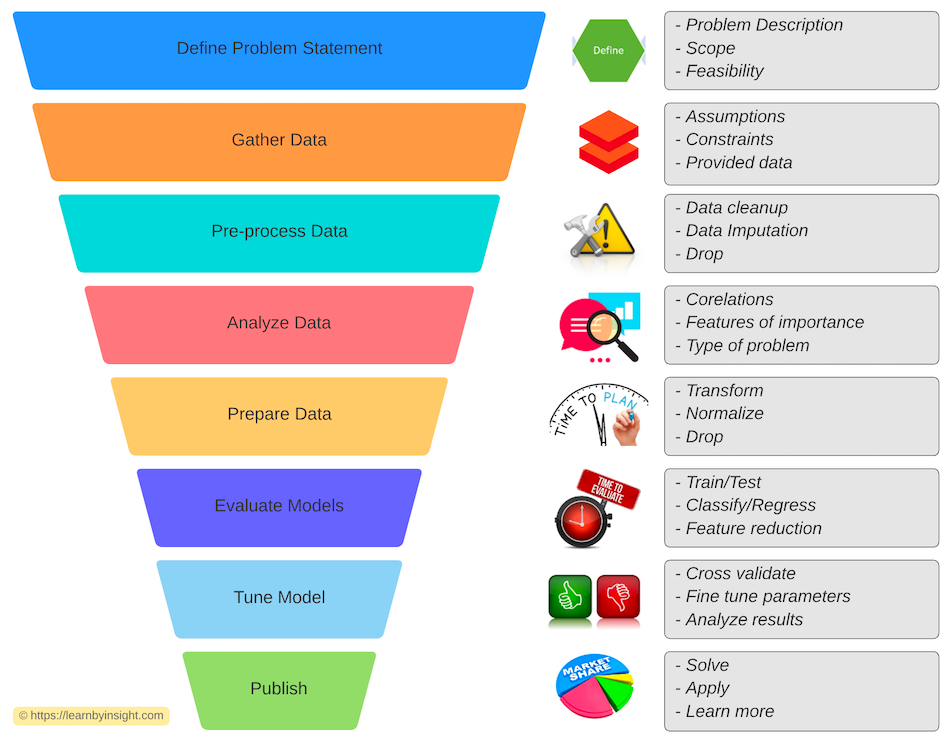
\includegraphics[width=0.75\textwidth]{media/ml-workflow.png}
        \caption{Machine Learning workflow~\cite{Mewara2020}}
    \end{figure}
\end{frame}